\documentclass[10pt]{beamer}
\beamertemplatenavigationsymbolsempty
\usecolortheme{beaver}
\setbeamertemplate{blocks}[rounded=true, shadow=true]
%\setbeamertemplate{footline}[page number]
%
\usepackage[utf8]{inputenc}
\usepackage[english,russian]{babel}
\usepackage{amssymb,amsfonts,amsmath,mathtext}
\usepackage{subfig}
\usepackage[all]{xy} % xy package for diagrams
\usepackage{array}
\usepackage{multicol}% many columns in slide
\usepackage{hyperref}% urls
\usepackage{hhline}%tables

\usepackage{caption}
\usepackage{subfig} % for subfigures

\DeclareMathOperator*{\argmax}{arg\,max}  % in your preamble
\DeclareMathOperator*{\argmin}{arg\,min}  % in your preamble 

% Your figures are here:
\graphicspath{ {../figures/} }

%----------------------------------------------------------------------------------------------------------
\title[\hbox to 56mm{Восстановление снимков фМРТ}]{Восстановление снимков фМРТ \\ по просматриваемому видеоряду}
\author[Н.\,С.~Киселев]{Никита Сергеевич Киселев}
\institute{Московский физико-технический институт}
\date{\footnotesize
\par\smallskip\emph{Курс:} Автоматизация научных исследований\par/Группа 003
\par\smallskip\emph{Эксперт:} А.\,В.~Грабовой
\par\bigskip\small 2023}
%----------------------------------------------------------------------------------------------------------
\begin{document}
%----------------------------------------------------------------------------------------------------------
\begin{frame}{Восстановление снимков фМРТ по видеоряду}

\textcolor{red}{Цель эксперимента:} выбор оптимального метода восстановления снимков фМРТ по видеоряду,
просматриваемому человеком

\textcolor{red}{Метод:} построение линейной модели для каждого вокселя в отдельности,
подбор гиперпараметра времени задержки $\Delta t$

\vspace{-0.5cm}

\begin{columns}[c]
    \column{0.45\textwidth}
        \begin{figure}[h!]
            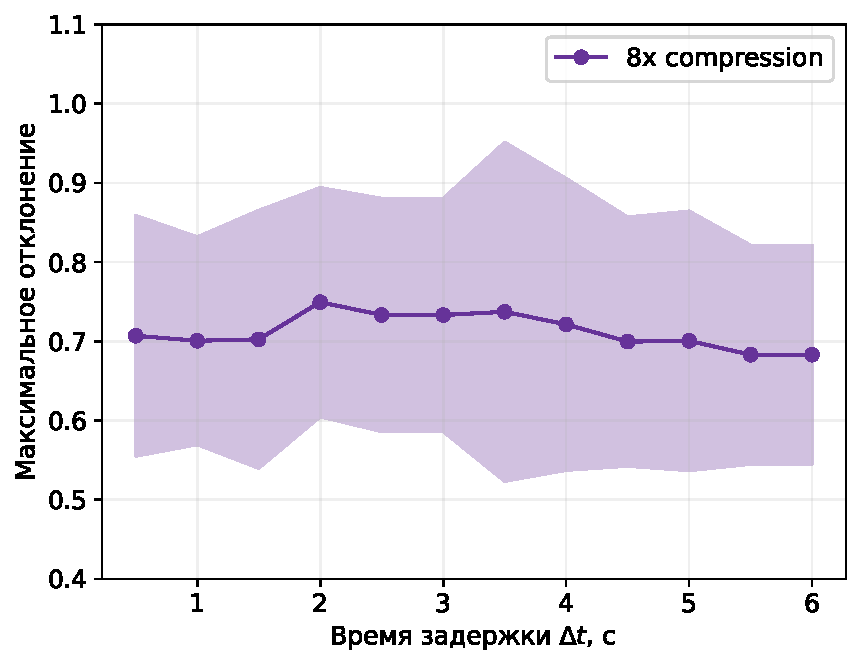
\includegraphics[width=1.0\textwidth]{subs_deviation_dt.pdf}
        \end{figure}
    \column{0.55\textwidth}
        \begin{figure}[h!]
            \centering
            \subfloat[Истинный снимок]{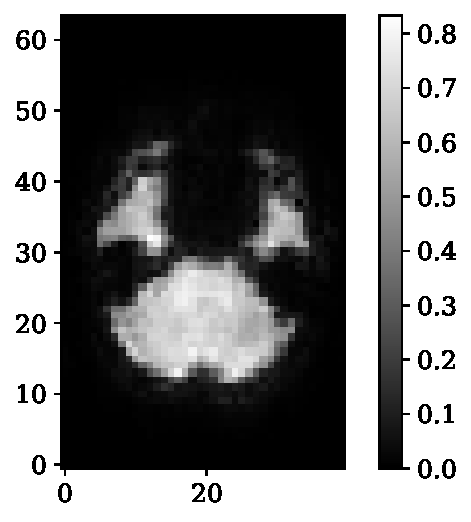
\includegraphics[width=0.5\textwidth]{sub-4-04-1/sub-4-04-1-_-_-32-orig.pdf}}
            \hfill
            \subfloat[Разность]{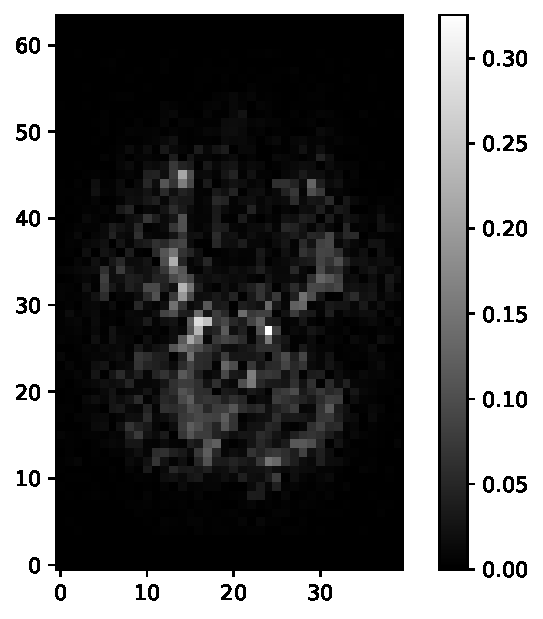
\includegraphics[width=0.5\textwidth]{sub-4-04-1/sub-4-04-1-_-_-32-delta.pdf}}
        \end{figure}
\end{columns}

\[ \hat{\mathbf{w}}_{ijk} = \argmin_{\mathbf{w}_{ijk}} \sum\limits_{\ell = 1}^{N_{\mathbf{S}} - \mu \Delta t} \big( \langle \mathbf{x}_{\ell}, \mathbf{w}_{ijk} \rangle - v^{\ell}_{ijk} \big)^2 \]

\vspace{-0.1cm}

$\mathbf{x}_{\ell}$~--- векторное описание изображение, $v^{\ell}_{ijk}$~--- значение вокселя снимка фМРТ,
$N_{\mathbf{S}}$~--- количество снимков фМРТ, $\mu$~--- их частота, 
$\Delta t$~--- гиперпараметр, время задержки

\end{frame}

\end{document} 